% ============================================================
%  يُترجَم بـ XeLaTeX  (في Overleaf: Menu → Compiler → XeLaTeX)
%  الخط: Amiri (متوفر في Overleaf، أو حمّله من github.com/aliftype/amiri)
% ============================================================
\documentclass[12pt,a4paper]{article}
\usepackage[a4paper,margin=1.7cm,top=2.3cm,bottom=2.9cm,headheight=15pt,footskip=1.5cm]{geometry}
\usepackage{amsmath,amssymb}
\usepackage{icomma}
\usepackage[english,bidi=default,layout=lists]{babel}
\babelprovide[import,main]{arabic}
\babelfont{rm}[Scale=1.08]{Amiri}
\babelfont{sf}[Scale=1.08]{Amiri}
\usepackage[most]{tcolorbox}
\usepackage{tikz}
\usetikzlibrary{arrows.meta,calc,shadings}
\usepackage{array}
\usepackage{colortbl}
\usepackage{fancyhdr}
\usepackage{titlesec}
\usepackage{enumitem}
\usepackage{collcell}
\usepackage{needspace}
\usepackage{etoolbox}
\newcolumntype{C}{>{\collectcell\ar}c<{\endcollectcell}}
\pretocmd{\section}{\Needspace{15\baselineskip}}{}{}
\pretocmd{\subsection}{\Needspace{11\baselineskip}}{}{}

\definecolor{cDef}{HTML}{1F4E9C}
\definecolor{cThm}{HTML}{B3261E}
\definecolor{cRem}{HTML}{2E7D32}
\definecolor{cEx}{HTML}{C76B00}
\definecolor{cMeth}{HTML}{6A1B9A}
\definecolor{cSol}{HTML}{00695C}
\definecolor{cSec}{HTML}{1F3A68}

\titleformat{\section}{\Large\bfseries\color{cSec}}{\thesection.}{0.6em}{}[{\color{cSec!60}\titlerule[1pt]}]
\titleformat{\subsection}{\large\bfseries\color{cThm!85!black}}{\thesubsection.}{0.5em}{}
\titlespacing*{\section}{0pt}{14pt}{8pt}
\titlespacing*{\subsection}{0pt}{10pt}{5pt}
\setlength{\parindent}{0pt}
\setlength{\parskip}{4pt}
\setlist{itemsep=2pt,topsep=3pt}

\newtcolorbox{arbox}[3][]{enhanced,
  colback=#2!5,colframe=#2!80!black,arc=2mm,boxrule=0.8pt,
  left=6pt,right=6pt,top=8pt,bottom=5pt,
  fonttitle=\bfseries,coltitle=white,
  title={\foreignlanguage{arabic}{#3}},
  attach boxed title to top right={xshift=-5mm,yshift=-3mm},
  boxed title style={colback=#2!80!black,arc=1.5mm,boxrule=0pt},
  before upper={\selectlanguage{arabic}},
  before skip=8pt,after skip=8pt,breakable,#1}
\newenvironment{BOX}[2]{\begin{otherlanguage}{english}\begin{arbox}{#1}{#2}}{\end{arbox}\end{otherlanguage}}
\newenvironment{tarif}[1][تعريف]{\begin{BOX}{cDef}{#1}}{\end{BOX}}
\newenvironment{khassia}[1][خاصية]{\begin{BOX}{cThm}{#1}}{\end{BOX}}
\newenvironment{molahada}[1][ملاحظة]{\begin{BOX}{cRem}{#1}}{\end{BOX}}
\newenvironment{mithal}[1][مثال]{\begin{BOX}{cEx}{#1}}{\end{BOX}}
\newenvironment{tariqa}[1][طريقة]{\begin{BOX}{cMeth}{#1}}{\end{BOX}}

\newcounter{exo}
\newenvironment{tamrin}[1]{\stepcounter{exo}\begin{BOX}{cSec}{التمرين \theexo: #1}}{\end{BOX}}
\newenvironment{hal}{\Needspace{12\baselineskip}\begin{otherlanguage}{english}\begin{arbox}[breakable]{cSol}{حل التمرين \theexo}}{\end{arbox}\end{otherlanguage}}

\newenvironment{LTR}{\begin{otherlanguage}{english}}{\end{otherlanguage}}
\newcommand{\ar}[1]{\foreignlanguage{arabic}{#1}}

\renewcommand{\dots}{\mathinner{\ldotp\ldotp\ldotp}}
\renewcommand{\ldots}{\mathinner{\ldotp\ldotp\ldotp}}
\renewcommand{\cdots}{\mathinner{\cdotp\cdotp\cdotp}}
\newcommand{\N}{\mathbb{N}}
\newcommand{\Z}{\mathbb{Z}}
\newcommand{\D}{\mathbb{D}}
\newcommand{\Q}{\mathbb{Q}}
\newcommand{\R}{\mathbb{R}}
\newcommand{\pgcd}{\operatorname{PGCD}}
\newcommand{\ppcm}{\operatorname{PPCM}}

% \NLseg{a}{b}{[}{]} ; \NLright{a}{[} ; \NLleft{b}{]}  (interval on a number line)
\newcommand{\NLseg}[4]{\begin{LTR}\begin{tikzpicture}[baseline=-0.6ex]
 \draw[-{Stealth[length=2mm]},gray!70](0,0)--(3.4,0);
 \draw[line width=2pt,cThm!80!black](0.7,0)--(2.7,0);
 \node[cThm!80!black,font=\LARGE] at (0.7,0){$#3$};
 \node[cThm!80!black,font=\LARGE] at (2.7,0){$#4$};
 \node[below=3pt,font=\footnotesize] at (0.7,0){$#1$};
 \node[below=3pt,font=\footnotesize] at (2.7,0){$#2$};
\end{tikzpicture}\end{LTR}}
\newcommand{\NLright}[2]{\begin{LTR}\begin{tikzpicture}[baseline=-0.6ex]
 \draw[-{Stealth[length=2mm]},gray!70](0,0)--(3.4,0);
 \draw[line width=2pt,cThm!80!black](1.3,0)--(3.3,0);
 \node[cThm!80!black,font=\LARGE] at (1.3,0){$#2$};
 \node[below=3pt,font=\footnotesize] at (1.3,0){$#1$};
\end{tikzpicture}\end{LTR}}
\newcommand{\NLleft}[2]{\begin{LTR}\begin{tikzpicture}[baseline=-0.6ex]
 \draw[-{Stealth[length=2mm]},gray!70](0,0)--(3.4,0);
 \draw[line width=2pt,cThm!80!black](0.05,0)--(2.1,0);
 \node[cThm!80!black,font=\LARGE] at (2.1,0){$#2$};
 \node[below=3pt,font=\footnotesize] at (2.1,0){$#1$};
\end{tikzpicture}\end{LTR}}

% ---------- social-media icons (pure TikZ) ----------
\definecolor{cFB}{HTML}{1877F2}
\definecolor{cTG}{HTML}{229ED9}
\definecolor{cIG1}{HTML}{FEDA75}
\definecolor{cIG2}{HTML}{D62976}
\definecolor{cIG3}{HTML}{4F5BD5}
\newcommand{\fbicon}{\begin{LTR}\begin{tikzpicture}[baseline=-0.75ex,x=1em,y=1em]
 \fill[cFB] (0,0) circle (0.55);
 \node[white,inner sep=0,font=\usefont{TU}{lmss}{bx}{n}\small] at (0.04,-0.02) {f};
\end{tikzpicture}\end{LTR}}
\newcommand{\igicon}{\begin{LTR}
\begin{tikzpicture}[baseline=-0.75ex,x=1em,y=1em]
 \shade[lower left=cIG1,lower right=cIG2,upper left=cIG2,upper right=cIG3,rounded corners=0.28em] (-0.55,-0.55) rectangle (0.55,0.55);
 \draw[white,line width=0.09em,rounded corners=0.18em] (-0.36,-0.36) rectangle (0.36,0.36);
 \draw[white,line width=0.09em] (0,0) circle (0.17);
 \fill[white] (0.22,0.22) circle (0.05);
\end{tikzpicture}\end{LTR}}
\newcommand{\tgicon}{\begin{LTR}
\begin{tikzpicture}[baseline=-0.75ex,x=1em,y=1em]
 \fill[cTG] (0,0) circle (0.55);
 \fill[white] (-0.33,0.0) -- (0.32,0.27) -- (0.2,-0.3) -- (0.0,-0.15) -- (-0.08,-0.28) -- (-0.08,-0.08) -- cycle;
 \fill[cTG!70!black] (-0.08,-0.08) -- (0.25,0.2) -- (0.0,-0.15) -- (-0.08,-0.28) -- cycle;
\end{tikzpicture}\end{LTR}}
% page number: black box, white two-digit number, at the right of the social row
\newcommand{\PageBox}{\begin{LTR}\tikz[baseline=(p.base)]\node[fill=black,text=white,inner sep=2.5pt,minimum width=1.6em,minimum height=1.3em,font=\usefont{TU}{lmss}{bx}{n}\small](p){\ifnum\value{page}<10 0\fi\arabic{page}};\end{LTR}}
% visual left-to-right order: Telegram | Instagram | Facebook | page box
\newcommand{\SocialRow}{\begin{otherlanguage}{english}%
 \ar{\textbf{الأستاذ سوايسية هشام للرياضيات}}\ \tgicon\hfill
 \textbf{prof\_hicham\_math}\ \igicon\hfill
 \ar{\textbf{الأستاذ سوايسية هشام للرياضيات}}\ \fbicon\hspace{2.2em}\PageBox\end{otherlanguage}}

\pagestyle{fancy}
\fancyhf{}
\renewcommand{\headrulewidth}{0.6pt}
\renewcommand{\footrulewidth}{0.4pt}
% \SetHeader{right head: document title}{left head: level -- stream}
\newcommand{\SetHeader}[2]{%
 \fancyhead[C]{\parbox{\textwidth}{\ar{#1\hfill #2}}}%
 \fancyfoot[C]{\parbox{\textwidth}{\small\SocialRow}}}
\usepackage{tkz-tab}
\usepackage{multicol}
% variation / sign table (LTR)
\newenvironment{TAB}{\par\begin{center}\begin{LTR}\begin{tikzpicture}[scale=0.95,every node/.style={font=\small}]}{\end{tikzpicture}\end{LTR}\end{center}}
% grid + axes, clipped: \begin{GR}{xmin}{xmax}{ymin}{ymax}{unit cm}
\newenvironment{GR}[5]{\par\begin{center}\begin{LTR}\begin{tikzpicture}[x=#5cm,y=#5cm,font=\footnotesize]
 \draw[gray!25,very thin] (#1,#3) grid (#2,#4);
 \draw[-{Stealth[length=2mm]}] (#1,0)--(#2+0.3,0) node[below left]{$x$};
 \draw[-{Stealth[length=2mm]}] (0,#3)--(0,#4+0.3) node[below left]{$y$};
 \node[below left] at (0,0){$O$};
 \begin{scope}\clip (#1,#3) rectangle (#2,#4);}
{\end{scope}\end{tikzpicture}\end{LTR}\end{center}}
\newcommand{\Ticks}[2]{\foreach \t in {#1} \node[below,font=\scriptsize] at (\t,0){$\t$}; \foreach \t in {#2} \node[left,font=\scriptsize] at (0,\t){$\t$};}
\newcommand{\bx}[1]{\ensuremath{\colorbox{cDef!12}{$\displaystyle #1$}}}
\newcommand{\TwoCol}[4]{\par\begin{LTR}\noindent\begin{minipage}[t]{#1\textwidth}\selectlanguage{arabic}#2\end{minipage}\hfill\begin{minipage}[t]{#3\textwidth}\selectlanguage{arabic}#4\end{minipage}\end{LTR}\par}
\newcommand{\RL}[4]{\TwoCol{#3}{#4}{#1}{#2}}  % \RL{w1}{right content}{w2}{left content}
\newcommand{\ok}{$\textcolor{cRem}{\checkmark}$}
\newcommand{\limn}{\displaystyle\lim_{n\to+\infty}}
% sub-questions, each on its own line
\newenvironment{sq}{\begin{itemize}[leftmargin=2.4em,itemsep=3pt]}{\end{itemize}}
\newcommand{\qa}{\item[(أ)]}\newcommand{\qb}{\item[(ب)]}\newcommand{\qc}{\item[(جـ)]}\newcommand{\qd}{\item[(د)]}\newcommand{\qe}{\item[(هـ)]}
\newcommand{\pa}{\par\smallskip\textbf{(أ)} }\newcommand{\pb}{\par\smallskip\textbf{(ب)} }\newcommand{\pc}{\par\smallskip\textbf{(جـ)} }\newcommand{\pd}{\par\smallskip\textbf{(د)} }\newcommand{\pe}{\par\smallskip\textbf{(هـ)} }
\newcommand{\QQ}[1]{\par\smallskip\textbf{#1.} }
\newenvironment{tmr}{\stepcounter{exo}\begin{BOX}{cSec}{تمرين محلول \theexo}}{\end{BOX}}
\newcommand{\ABC}[3]{\\[2pt]\begin{tabular}{p{0.28\textwidth}p{0.28\textwidth}p{0.28\textwidth}}(جـ) \ #3 & (ب) \ #2 & (أ) \ #1\end{tabular}}
\pretocmd{\section}{\Needspace{24\baselineskip}}{}{}
\newtcbox{\bxtbox}{on line,colback=cDef!12,colframe=cDef!12,boxrule=0pt,arc=1pt,boxsep=0pt,left=2pt,right=2pt,top=1pt,bottom=1pt}
\newcommand{\bxt}[1]{\foreignlanguage{english}{\bxtbox{\ar{#1}}}}
\usepackage{longtable}
\setlength{\LTpre}{4pt}\setlength{\LTpost}{0pt}
\newcommand{\Phase}[1]{\textbf{#1}}
\newcommand{\Fld}[2]{\textbf{#1:}\ #2}
% رأس المذكرة على نمط النموذج: إطار بعنوان «مذكرة رقم»، معلومات الحصة، ثم إطار الكفاءات
\newcommand{\ModhHead}[9]{%
\begin{LTR}
\begin{tcolorbox}[enhanced,colback=white,colframe=cThm!85!black,arc=4mm,boxrule=1pt,top=14pt,bottom=6pt,left=8pt,right=8pt,
 overlay={\node[fill=cThm!85!black,text=white,rounded corners=3mm,inner xsep=14pt,inner ysep=4pt,font=\large\bfseries] at ([yshift=0pt]frame.north){\ar{مذكرة رقم #1}};},
 before upper={\selectlanguage{arabic}}]
\begin{tabular}{@{}p{0.4\linewidth}p{0.55\linewidth}@{}}
\Fld{المستوى}{#2} & \Fld{الثانوية}{\dotfill}\\[3pt]
\Fld{المادة}{رياضيات} & \Fld{ميدان التعلم}{#3}\\[3pt]
\Fld{المدة}{#5} & \Fld{الوحدة التعلمية}{#4}\\[3pt]
\Fld{الأستاذ}{\dotfill} & \Fld{المحتوى المعرفي}{#6}\\
\end{tabular}
\end{tcolorbox}
\begin{tcolorbox}[enhanced,colback=white,colframe=cThm!85!black,arc=3mm,boxrule=0.8pt,sidebyside,sidebyside align=top,lefthand ratio=0.5,
 segmentation style={dashed,cThm!60},before upper={\selectlanguage{arabic}},before lower={\selectlanguage{arabic}}]
\textbf{الكفاءات المستهدفة:}\par #8
\tcblower
\textbf{الكفاءات القبلية:}\par #7
\end{tcolorbox}
\end{LTR}
\par\smallskip\textbf{الوسائل:} #9\par\smallskip}
\newenvironment{Sayr}{%
\begin{LTR}\renewcommand{\arraystretch}{1.25}
\begin{longtable}{|p{0.17\textwidth}|>{\centering\arraybackslash}p{0.06\textwidth}|p{0.53\textwidth}|>{\centering\arraybackslash}p{0.12\textwidth}|}
\hline\rowcolor{cThm!12}\ar{\textbf{توجيهات وتعاليق}} & \ar{\textbf{المدة}} & \ar{\textbf{سير الحصة}} & \ar{\textbf{مراحل الحصة}}\\\hline\endhead
\hline\endfoot}{\end{longtable}\end{LTR}}
% سطر في الجدول: \Row{مرحلة}{سير}{مدة}{توجيهات}
\newcommand{\Row}[4]{\ar{\small #4} & \ar{#3} & \ar{#2} & \cellcolor{cThm!8}\ar{\Phase{#1}}\\\hline}

\newcommand{\Lab}[2]{\foreignlanguage{english}{\tcbox[on line,colback=#1,colframe=#1,boxrule=0pt,arc=2pt,boxsep=1pt,left=5pt,right=5pt,top=1pt,bottom=1pt]{\ar{\textcolor{white}{\textbf{#2}}}}}}
\newcommand{\Num}[1]{\foreignlanguage{english}{\tikz[baseline=(c.base)]\node[fill=cDef,text=white,inner sep=2pt,font=\footnotesize\bfseries](c){#1};}}
\newcommand{\ck}{\ensuremath{{\color{cRem}\checkmark}}}
\newenvironment{Kad}[1]{\par\smallskip\Lab{#1}}{\par}
\SetHeader{\small\bfseries\color{cSec}مذكرات محور: الدوال}{\small\color{cSec}السنة الثانية ثانوي -- علوم تجريبية}
\begin{document}
\begin{LTR}
\begin{tcolorbox}[enhanced,colback=cThm!85!black,colframe=cThm!85!black,arc=3mm,halign=center,boxrule=0pt,top=12pt,bottom=12pt,before upper={\selectlanguage{arabic}}]
{\color{white}\fontsize{26}{32}\selectfont\bfseries مذكرات محور: الدوال}\\[8pt]
{\color{white}\large السنة الثانية ثانوي -- علوم تجريبية (صالحة لشعبتي رياضيات وتقني رياضي)}\\[4pt]
{\color{white}\large 9 مذكرات (18 ساعة) -- السنة الدراسية 2026-2027}
\end{tcolorbox}
\end{LTR}
\begin{BOX}{cThm}{يتضمن هذا العمل}
\begin{enumerate}[label=\textbf{مذكرة \arabic{enumi}:},leftmargin=6em]
\item تذكير حول الدوال والدوال المرجعية.
\item العمليات على الدوال ومقارنة دالتين.
\item تركيب دالتين وتفكيك دالة.
\item اتجاه تغير الدوال $u+k$ ، $\lambda u$ ، $\sqrt u$ ، $\frac1u$ ، $g\circ u$.
\item التمثيلات البيانية المستنتجة.
\item محور تناظر ومركز تناظر منحنٍ.
\item كثيرات الحدود: الدرجة ، التساوي ، الجذور والتحليل.
\item القسمة الإقليدية لكثيرات الحدود وجدول هورنر.
\item المعادلات والمتراجحات من الدرجة الثانية والثالثة.
\end{enumerate}
مراجع النشاطات: الكتاب المدرسي للسنة الثانية ثانوي (باب الدوال العددية ص 8--9 ، باب كثيرات الحدود ص 36--37).
\end{BOX}
\newpage
\ModhHead{01}{2 ع ت}{تحليل}{الدوال}{02 سا}{تذكير حول الدوال والدوال المرجعية}%
{\begin{itemize}\item مفهوم الدالة ، الصورة والسابقة (1 ج م).\item الدوال المرجعية (1 ج م).\end{itemize}}%
{\begin{itemize}\item تعيين مجموعة تعريف دالة.\item استعمال خواص الدوال المرجعية وتمثيلاتها.\end{itemize}}%
{المنهاج ، الكتاب المدرسي ، مراجع ، الحاسبة البيانية.}
\begin{Sayr}
\Row{مرحلة الانطلاق}{%
\textbf{التهيئة النفسية:} أعطِ دالة تعرفها من السنة الأولى ، ارسم شكل منحناها بسرعة.}{10 د}{رسم سريع على السبورة.}
\Row{التشخيص والاكتشاف}{%
\Lab{cEx}{مناقشة نشاط 01 صفحة 8}\par\ck\ قراءة بيانية: صور أعداد ، حل معادلات $f(x)=k$ ومتراجحات $f(x)<k$.\par
\ck\ تشكيل جدول التغيرات وتعيين القيم الحدية من المنحني.\par
\ck\ نُذكّر أن حلول $f(x)=k$ هي فواصل نقط تقاطع $C_f$ مع المستقيم $y=k$.\par
}{35 د}{عمل ثنائي على المنحني.}
\Row{بناء المعارف}{%
\Lab{cDef}{مجموعة التعريف}\ مجموعة الأعداد الحقيقية $x$ التي يكون من أجلها حساب $f(x)$ ممكناً.\par\Lab{cMeth}{طريقة}\par\ck\ كسر: المقام لا ينعدم.\par
\ck\ جذر تربيعي: ما تحت الجذر موجب.\par
}{50 د}{جدول ملخص يُنقل في الكراس.}
\Row{}{%
\Lab{cEx}{مثال}\ $f(x)=\dfrac{\sqrt{x-1}}{x-3}$: نشترط $x-1\geqslant0$ و $x\neq3$ ، إذن $D_f=[1;3[\cup]3;+\infty[$.\par\Lab{cDef}{اتجاه التغير}\ $f$ متزايدة تماماً على $I$ معناه: من أجل $a<b$ من $I$ يكون $f(a)<f(b)$ (ومتناقصة تماماً: $f(a)>f(b)$).\par}{}{}
\Row{}{%
\Lab{cThm}{الدوال المرجعية}\par\smallskip\begin{LTR}\centering {\footnotesize\renewcommand{\arraystretch}{1.4}\begin{tabular}{|c|c|c|c|}\hline
\rowcolor{cSec!12}\ar{الدالة} & \ar{مجموعة التعريف} & \ar{متناقصة على} & \ar{متزايدة على}\\\hline
$x\mapsto x^2$ & $\mathbb R$ & $]-\infty;0]$ & $[0;+\infty[$\\\hline
$x\mapsto x^3$ & $\mathbb R$ & $-$ & $\mathbb R$\\\hline
$x\mapsto \dfrac1x$ & $\mathbb R^*$ & $]-\infty;0[$ \ar{و} $]0;+\infty[$ & $-$\\\hline
$x\mapsto\sqrt x$ & $[0;+\infty[$ & $-$ & $[0;+\infty[$\\\hline
$x\mapsto|x|$ & $\mathbb R$ & $]-\infty;0]$ & $[0;+\infty[$\\\hline
\end{tabular}}\end{LTR}\par \Lab{cRem}{ملاحظات}\ الدالتان $x\mapsto x^2$ و $x\mapsto|x|$ زوجيتان ؛ $x\mapsto x^3$ و $x\mapsto\frac1x$ فرديتان.}{}{}
\Row{التقويم}{%
\Lab{cEx}{تطبيق}\par عيّن مجموعة تعريف: $g(x)=\dfrac1{x^2-4}$ ؛ $h(x)=\sqrt{2-x}$.\par\textbf{الحل:} $D_g=\mathbb R-\{-2;2\}$ ؛ $D_h=]-\infty;2]$.\par\textbf{واجب منزلي:} تمارين من الكتاب المدرسي.\par\smallskip\textbf{ملاحظات حول سير الحصة:} \dotfill}{25 د}{تقويم فردي.}
\end{Sayr}
\newpage
\ModhHead{02}{2 ع ت}{تحليل}{الدوال}{02 سا}{العمليات على الدوال: المجموع ، الجداء ، حاصل القسمة ، مقارنة دالتين}%
{\begin{itemize}\item الدوال المرجعية.\end{itemize}}%
{\begin{itemize}\item تعيين مجموع وجداء وحاصل قسمة دالتين ومجموعة تعريفها.\item مقارنة دالتين جبرياً وبيانياً.\end{itemize}}%
{المنهاج ، الكتاب المدرسي ، مراجع ، الحاسبة البيانية.}
\begin{Sayr}
\Row{مرحلة الانطلاق}{%
\textbf{التهيئة النفسية:} سعر $x$ كلغ من البرتقال $f(x)$ وسعر $x$ كلغ من التفاح $g(x)$: ماذا يمثل $f(x)+g(x)$ ؟}{10 د}{وضعية من الحياة.}
\Row{التشخيص والاكتشاف}{%
\Lab{cEx}{مناقشة نشاط 03 صفحة 8}\par\ck\ رسم منحنيين على ورق ميليمتري ، واستنتاج حلول معادلة $f(x)=g(x)$ بيانياً: فواصل نقط التقاطع.\par
\ck\ التحقق بالحساب.\par
}{35 د}{ورق ميليمتري.}
\Row{بناء المعارف}{%
\Lab{cDef}{تعريف}\ $f$ و $g$ دالتان معرفتان على $D$ ، $\lambda$ عدد حقيقي:\par\ck\ $(f+g)(x)=f(x)+g(x)$ ، $(\lambda f)(x)=\lambda f(x)$ ، $(f\times g)(x)=f(x)\times g(x)$.\par
\ck\ $\left(\dfrac fg\right)(x)=\dfrac{f(x)}{g(x)}$ معرفة حيث $g(x)\neq0$.\par
\Lab{cDef}{تساوي ومقارنة دالتين}\par\ck\ $f=g$ معناه: لهما نفس مجموعة التعريف $D$ و $f(x)=g(x)$ لكل $x$ من $D$.\par
\ck\ $f\leqslant g$ على $I$ معناه $f(x)\leqslant g(x)$ لكل $x$ من $I$: $C_f$ تحت $C_g$.\par
}{50 د}{نرسم المنحنيين لتأكيد النتيجة.}
\Row{}{%
\Lab{cMeth}{دراسة الوضع النسبي}\ ندرس إشارة الفرق $f(x)-g(x)$.\par\Lab{cEx}{مثال}\ $f(x)=x^2$ ، $g(x)=2x-1$: $f(x)-g(x)=(x-1)^2\geqslant0$ ، إذن $C_f$ فوق $C_g$ ويتقاطعان في النقطة $(1;1)$.\par}{}{}
\Row{}{%
\Lab{cThm!80!black}{حذار}\ الدالتان $x\mapsto\dfrac{x^2}x$ و $x\mapsto x$ غير متساويتين (مجموعتا التعريف مختلفتان).}{}{}
\Row{التقويم}{%
\Lab{cEx}{تطبيق}\par قارن الدالتين $f(x)=x$ و $g(x)=x^2$ على المجال $[0;1]$.\par\textbf{الحل:} $f(x)-g(x)=x(1-x)\geqslant0$ على $[0;1]$ ، إذن $x^2\leqslant x$ و $C_g$ تحت $C_f$.\par\textbf{واجب منزلي:} تمارين من الكتاب المدرسي.\par\smallskip\textbf{ملاحظات حول سير الحصة:} \dotfill}{25 د}{تقويم فردي.}
\end{Sayr}
\newpage
\ModhHead{03}{2 ع ت}{تحليل}{الدوال}{02 سا}{تركيب دالتين وتفكيك دالة}%
{\begin{itemize}\item العمليات على الدوال.\end{itemize}}%
{\begin{itemize}\item تعيين مركب دالتين ومجموعة تعريفه.\item تفكيك دالة إلى مركب دوال مرجعية.\end{itemize}}%
{المنهاج ، الكتاب المدرسي ، مراجع ، الحاسبة البيانية.}
\begin{Sayr}
\Row{مرحلة الانطلاق}{%
\textbf{التهيئة النفسية:} آلة أولى تضاعف العدد ، وآلة ثانية تضيف له $3$: ماذا نحصل إذا مررنا العدد بالآلتين؟ وهل يهم الترتيب؟}{10 د}{مثال الآلتين.}
\Row{التشخيص والاكتشاف}{%
\Lab{cEx}{مناقشة نشاط 05 صفحة 9}\par\ck\ $x$ بدلالة الزمن $t$ ، والمسافة بدلالة $x$: المرور من $t$ إلى المسافة يتم بإتباع المخطط $t\mapsto x\mapsto d$.\par
\ck\ نسمي الدالة الناتجة \textbf{مركب دالتين}.\par
}{35 د}{نشاط من الكتاب.}
\Row{بناء المعارف}{%
\Lab{cDef}{تعريف}\ $(g\circ f)(x)=g\big(f(x)\big)$ ، وهي معرفة إذا كان $x\in D_f$ و $f(x)\in D_g$.\par\Lab{cEx}{مثال}\ $f(x)=x-3$ و $g(x)=\sqrt x$:\par\ck\ $(g\circ f)(x)=\sqrt{x-3}$ معرفة على $[3;+\infty[$.\par
\ck\ $(f\circ g)(x)=\sqrt x-3$ معرفة على $[0;+\infty[$.\par
}{50 د}{نكتب المخطط بالأسهم.}
\Row{}{%
\Lab{cThm!80!black}{حذار}\ عموماً $g\circ f\neq f\circ g$.\par\Lab{cMeth}{تفكيك دالة}\ نبحث عن العمليات المتتالية التي نطبقها على $x$.\par}{}{}
\Row{}{%
\Lab{cEx}{مثال}\par\ck\ $h(x)=(2x-1)^2$: $x\overset{u}{\longmapsto}2x-1\overset{v}{\longmapsto}(2x-1)^2$ ، إذن $h=v\circ u$ مع $u(x)=2x-1$ و $v(x)=x^2$.\par
\ck\ $k(x)=\dfrac3{x-2}+1$: $x\mapsto x-2\mapsto\dfrac1{x-2}\mapsto\dfrac3{x-2}\mapsto\dfrac3{x-2}+1$.\par
}{}{}
\Row{التقويم}{%
\Lab{cEx}{تطبيق}\par فكّك الدالة $k(x)=\sqrt{x^2+1}$ ، ثم احسب $(f\circ g)(x)$ و $(g\circ f)(x)$ حيث $f(x)=x^2$ و $g(x)=x+1$.\par\textbf{الحل:} $k=v\circ u$ مع $u(x)=x^2+1$ و $v(x)=\sqrt x$ ؛ $(f\circ g)(x)=(x+1)^2$ ، $(g\circ f)(x)=x^2+1$.\par\textbf{واجب منزلي:} تمارين من الكتاب المدرسي.\par\smallskip\textbf{ملاحظات حول سير الحصة:} \dotfill}{25 د}{تقويم فردي.}
\end{Sayr}
\newpage
\ModhHead{04}{2 ع ت}{تحليل}{الدوال}{02 سا}{اتجاه تغير الدوال $u+k$ ، $\lambda u$ ، $\sqrt u$ ، $\frac1u$ ، $g\circ u$}%
{\begin{itemize}\item اتجاه التغير ، تركيب دالتين.\end{itemize}}%
{\begin{itemize}\item استنتاج اتجاه تغير دالة من اتجاه تغير دوال مرجعية.\end{itemize}}%
{المنهاج ، الكتاب المدرسي ، مراجع ، الحاسبة البيانية.}
\begin{Sayr}
\Row{مرحلة الانطلاق}{%
\textbf{التهيئة النفسية:} إذا كانت $u$ متزايدة ، ماذا نقول عن $-u$ ؟ عن $u+5$ ؟}{10 د}{سؤال شفهي.}
\Row{التشخيص والاكتشاف}{%
\Lab{cEx}{مناقشة نشاط 04 صفحة 9}\par\ck\ دالتان تآلفيتان $f$ و $g$: اتجاه تغير كل منهما ، ثم اتجاه تغير دوال مشكلة منهما.\par
\ck\ نلاحظ أن ضرب دالة في عدد سالب يعكس اتجاه التغير.\par
}{35 د}{عمل ثنائي.}
\Row{بناء المعارف}{%
\Lab{cThm}{خاصية}\ $u$ دالة رتيبة على مجال $I$:\par\ck\ $u+k$ لها نفس اتجاه تغير $u$.\par
\ck\ $\lambda u$: نفس الاتجاه إذا $\lambda>0$ ، وعكسه إذا $\lambda<0$.\par
\ck\ إذا كانت $u\geqslant0$ على $I$: $\sqrt u$ لها نفس اتجاه تغير $u$.\par
\ck\ إذا كانت $u$ لا تنعدم وتحافظ على إشارة ثابتة على $I$: $\dfrac1u$ لها عكس اتجاه تغير $u$.\par
\Lab{cThm}{مركب دالتين}\ إذا كانت $u$ رتيبة على $I$ و $g$ رتيبة على $J$ مع $u(x)\in J$: $g\circ u$ متزايدة إذا كان لهما نفس الاتجاه ، ومتناقصة إذا اختلف الاتجاهان.\par}{50 د}{نلخص القواعد في جدول.}
\Row{}{%
\Lab{cEx}{مثال}\par\ck\ $f(x)=\dfrac1{x-2}$ على $]2;+\infty[$: $u(x)=x-2$ متزايدة وموجبة ، إذن $f$ متناقصة.\par
\ck\ $f(x)=\sqrt{3-x}$ على $]-\infty;3]$: $u(x)=3-x$ متناقصة وموجبة ، إذن $f$ متناقصة.\par
\Lab{cThm!80!black}{حذار}\ القاعدة $\frac1u$ لا تُطبق على مجال تنعدم فيه $u$.}{}{}
\Row{التقويم}{%
\Lab{cEx}{تطبيق}\par ادرس اتجاه تغير $h(x)=-2(x-1)^2+3$ على $[1;+\infty[$.\par\textbf{الحل:} $x-1$ متزايدة وموجبة ، والدالة مربع متزايدة على $[0;+\infty[$ ، إذن $(x-1)^2$ متزايدة ؛ الضرب في $-2$ يعكس الاتجاه ، وإضافة $3$ لا تغيره: $h$ متناقصة على $[1;+\infty[$.\par\textbf{واجب منزلي:} تمارين من الكتاب المدرسي.\par\smallskip\textbf{ملاحظات حول سير الحصة:} \dotfill}{25 د}{تقويم فردي.}
\end{Sayr}
\newpage
\ModhHead{05}{2 ع ت}{تحليل}{الدوال}{02 سا}{التمثيلات البيانية المستنتجة}%
{\begin{itemize}\item الدوال المرجعية ، الأشعة والانسحاب (1 ج م).\end{itemize}}%
{\begin{itemize}\item رسم منحنيات الدوال $f(x+a)+b$ ، $-f$ ، $|f|$ انطلاقاً من $C_f$.\end{itemize}}%
{المنهاج ، الكتاب المدرسي ، مراجع ، الحاسبة البيانية. ورق ميليمتري.}
\begin{Sayr}
\Row{مرحلة الانطلاق}{%
\textbf{التهيئة النفسية:} ارسم منحني الدالة مربع ، ثم «حرّكه» دون تغيير شكله: ماذا يتغير في العبارة؟}{10 د}{سؤال بالرسم.}
\Row{التشخيص والاكتشاف}{%
\Lab{cEx}{وضعية مقترحة}\ ارسم في نفس المعلم منحنيي $x\mapsto x^2$ و $x\mapsto(x-2)^2+1$ بجدول قيم.\par\ck\ كل نقطة $M(x;x^2)$ ترفق بها النقطة $M_1(x+2;x^2+1)$: المنحني الثاني صورة الأول بالانسحاب الذي شعاعه $(2;1)$.\par
}{35 د}{جدول قيم وورق ميليمتري.}
\Row{بناء المعارف}{%
\Lab{cThm}{خاصية}\ $C_f$ منحني الدالة $f$ في معلم $(O;\vec i,\vec j)$:\par\ck\ منحني $x\mapsto f(x-a)+b$ صورة $C_f$ بالانسحاب الذي شعاعه $\vec w(a;b)$.\par
\ck\ منحني $-f$ نظير $C_f$ بالنسبة إلى محور الفواصل.\par
\ck\ منحني $|f|$: نحتفظ بجزء $C_f$ الذي فوق محور الفواصل ، ونأخذ نظير الجزء الذي تحته.\par
\Lab{cEx}{مثال}\ $f(x)=(x+1)^2-3$: $C_f$ صورة منحني الدالة مربع بالانسحاب الذي شعاعه $\vec w(-1;-3)$.\par\smallskip\begin{LTR}\centering 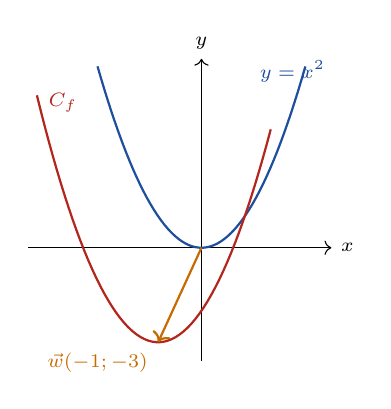
\begin{tikzpicture}[x=0.55cm,y=0.4cm,font=\scriptsize]
\draw[->] (-4,0)--(3,0) node[right]{$x$}; \draw[->] (0,-3.6)--(0,6) node[above]{$y$};
\draw[cDef,thick,domain=-2.4:2.4,samples=60] plot (\x,{\x*\x}); \node[cDef] at (2.1,5.6){$y=x^2$};
\draw[cThm,thick,domain=-3.8:1.6,samples=60] plot (\x,{(\x+1)*(\x+1)-3}); \node[cThm] at (-3.2,4.6){$C_f$};
\draw[->,thick,cEx] (0,0)--(-1,-3) node[below left]{$\vec w(-1;-3)$};
\end{tikzpicture}\end{LTR}\par }{50 د}{نتحقق بالحاسبة البيانية.}
\Row{}{%
\Lab{cEx}{دالة متجانسة}\ $g(x)=\dfrac{2x+3}{x+1}=2+\dfrac1{x+1}$: منحني $g$ صورة منحني $x\mapsto\frac1x$ بالانسحاب الذي شعاعه $(-1;2)$.\par\Lab{cThm!80!black}{حذار}\ في $f(x-a)$ يكون الانسحاب نحو اليمين إذا كان $a>0$.}{}{}
\Row{التقويم}{%
\Lab{cEx}{تطبيق}\par \Num{1} كيف نحصل على منحني $h(x)=\sqrt{x-1}+2$ ؟ \Num{2} ارسم منحني $x\mapsto|x^2-4|$.\par\textbf{الحل:} \Num{1} بالانسحاب الذي شعاعه $(1;2)$ لمنحني $\sqrt x$ ؛ \Num{2} نرسم $y=x^2-4$ ونأخذ نظير الجزء الواقع بين $-2$ و $2$ بالنسبة إلى محور الفواصل.\par\textbf{واجب منزلي:} تمارين من الكتاب المدرسي.\par\smallskip\textbf{ملاحظات حول سير الحصة:} \dotfill}{25 د}{تقويم فردي.}
\end{Sayr}
\newpage
\ModhHead{06}{2 ع ت}{تحليل}{الدوال}{02 سا}{محور تناظر ومركز تناظر منحنٍ}%
{\begin{itemize}\item الشفعية ، التمثيلات المستنتجة.\end{itemize}}%
{\begin{itemize}\item إثبات أن مستقيماً محور تناظر أو أن نقطة مركز تناظر لمنحنٍ.\end{itemize}}%
{المنهاج ، الكتاب المدرسي ، مراجع ، الحاسبة البيانية.}
\begin{Sayr}
\Row{مرحلة الانطلاق}{%
\textbf{التهيئة النفسية:} منحني الدالة مربع متناظر بالنسبة إلى محور التراتيب: لماذا؟ وماذا عن منحني $x\mapsto(x-2)^2$ ؟}{10 د}{سؤال شفهي.}
\Row{التشخيص والاكتشاف}{%
\Lab{cEx}{وضعية مقترحة}\ $f(x)=x^2-4x+1$. نضع $X=x-2$ و $Y=y+3$ (تغيير المبدأ إلى $\Omega(2;-3)$).\par\ck\ نجد $Y=X^2$: دالة زوجية في المعلم الجديد ، إذن المستقيم $x=2$ محور تناظر لـ $C_f$.\par
}{35 د}{تغيير المعلم.}
\Row{بناء المعارف}{%
\Lab{cThm}{خاصية}\par\ck\ المستقيم $x=a$ محور تناظر لـ $C_f$ إذا كان: من أجل كل $x$ من $D_f$ ، $(2a-x)\in D_f$ و $f(2a-x)=f(x)$.\par
\ck\ النقطة $\Omega(a;b)$ مركز تناظر لـ $C_f$ إذا كان: من أجل كل $x$ من $D_f$ ، $(2a-x)\in D_f$ و $f(2a-x)+f(x)=2b$.\par
\Lab{cEx}{مثال}\par\ck\ $f(x)=x^2-4x+1$: $f(4-x)=(4-x)^2-4(4-x)+1=x^2-4x+1=f(x)$ ، إذن $x=2$ محور تناظر.\par
\ck\ $g(x)=\dfrac{2x+3}{x+1}=2+\dfrac1{x+1}$: $g(-2-x)+g(x)=2-\dfrac1{x+1}+2+\dfrac1{x+1}=4$ ، إذن $\Omega(-1;2)$ مركز تناظر.\par
}{50 د}{الطريقتان على السبورة.}
\Row{}{%
\Lab{cThm!80!black}{حذار}\ نتحقق أولاً من أن $D_f$ متناظرة بالنسبة إلى $a$.\par\Lab{cRem}{ملاحظات}\ يمكن أيضاً استعمال تغيير المعلم $X=x-a$ ، $Y=y-b$ ثم دراسة شفعية الدالة الجديدة.}{}{}
\Row{التقويم}{%
\Lab{cEx}{تطبيق}\par \Num{1} بيّن أن $x=1$ محور تناظر لمنحني $f(x)=x^2-2x+3$. \Num{2} بيّن أن $\Omega(1;-1)$ مركز تناظر لمنحني $h(x)=x^3-3x^2+1$.\par\textbf{الحل:} \Num{1} $f(2-x)=x^2-2x+3=f(x)$ ؛ \Num{2} $h(2-x)+h(x)=-2=2\times(-1)$.\par\textbf{واجب منزلي:} تمارين من الكتاب المدرسي.\par\smallskip\textbf{ملاحظات حول سير الحصة:} \dotfill}{25 د}{تقويم فردي.}
\end{Sayr}
\newpage
\ModhHead{07}{2 ع ت}{تحليل}{الدوال}{02 سا}{كثيرات الحدود: الدرجة ، التساوي ، الجذور والتحليل}%
{\begin{itemize}\item النشر والتحليل ، الشكل النموذجي (1 ج م).\end{itemize}}%
{\begin{itemize}\item تعيين درجة كثير حدود ، وتطبيق مبدأ المطابقة.\item تحليل كثير حدود يقبل جذراً $\alpha$ إلى جداء $(x-\alpha)\,Q(x)$.\end{itemize}}%
{المنهاج ، الكتاب المدرسي ، مراجع ، الحاسبة البيانية.}
\begin{Sayr}
\Row{مرحلة الانطلاق}{%
\textbf{التهيئة النفسية:} هل العبارة $x^3-2x+\sqrt x$ كثير حدود؟ وهل $(x+1)^2-x^2$ من الدرجة $2$ ؟}{10 د}{سؤال تشخيصي.}
\Row{التشخيص والاكتشاف}{%
\Lab{cEx}{مناقشة النشاطين 01 و 02 صفحة 36}\par\ck\ نشر وترتيب عبارة كثير حدود ، وتعيين درجتها.\par
\ck\ اختيار الشكل المناسب (منشور ، محلل ، نموذجي) لحل معادلات.\par
}{35 د}{عمل ثنائي.}
\Row{بناء المعارف}{%
\Lab{cDef}{تعريف}\ $P(x)=a_nx^n+a_{n-1}x^{n-1}+\cdots+a_1x+a_0$ مع $a_n\neq0$: \textbf{درجته} $n$ ، و $a_n$ معامله الأعلى.\par\Lab{cThm}{تساوي كثيري حدود}\ يتساوى كثيرا حدود إذا وفقط إذا كانا من نفس الدرجة ومعاملات الحدود من نفس الدرجة متساوية (\textbf{مبدأ المطابقة}).\par}{50 د}{نكتب المطابقة في عمودين.}
\Row{}{%
\Lab{cDef}{الجذر}\ $\alpha$ جذر لـ $P$ إذا كان $P(\alpha)=0$.\par\Lab{cThm}{التحليل}\ إذا كان $\alpha$ جذراً لكثير حدود $P$ درجته $n\geqslant1$ ، فإن $P(x)=(x-\alpha)\,Q(x)$ حيث $Q$ كثير حدود درجته $n-1$.\par}{}{}
\Row{}{%
\Lab{cEx}{مثال}\ $P(x)=x^3-2x^2-5x+6$: $P(1)=0$. نضع $P(x)=(x-1)(ax^2+bx+c)=ax^3+(b-a)x^2+(c-b)x-c$.\par\ck\ بالمطابقة: $a=1$ ، $b-a=-2$ ، $c-b=-5$ ، $-c=6$ ، إذن $a=1$ ، $b=-1$ ، $c=-6$.\par
\ck\ $P(x)=(x-1)(x^2-x-6)=(x-1)(x+2)(x-3)$.\par
\Lab{cThm!80!black}{حذار}\ نتحقق دائماً من المعادلة الأخيرة ($-c=6$) لأنها تختبر صحة الجذر.}{}{}
\Row{التقويم}{%
\Lab{cEx}{تطبيق}\par $Q(x)=2x^3-3x^2-3x+2$. تحقق أن $2$ جذر لـ $Q$ ، ثم حلل $Q(x)$.\par\textbf{الحل:} $Q(2)=16-12-6+2=0$ ؛ بالمطابقة $Q(x)=(x-2)(2x^2+x-1)$ ؛ $\Delta=9$ ، والجذران $\frac12$ و $-1$: $Q(x)=(x-2)(2x-1)(x+1)$.\par\textbf{واجب منزلي:} تمارين من الكتاب المدرسي.\par\smallskip\textbf{ملاحظات حول سير الحصة:} \dotfill}{25 د}{تقويم فردي.}
\end{Sayr}
\newpage
\ModhHead{08}{2 ع ت}{تحليل}{الدوال}{02 سا}{القسمة الإقليدية لكثيرات الحدود وجدول هورنر}%
{\begin{itemize}\item الجذور والتحليل بـ $(x-\alpha)$.\end{itemize}}%
{\begin{itemize}\item إنجاز القسمة الإقليدية لكثير حدود على $(x-\alpha)$ بالطريقة المطولة وبجدول هورنر.\end{itemize}}%
{المنهاج ، الكتاب المدرسي ، مراجع ، الحاسبة البيانية.}
\begin{Sayr}
\Row{مرحلة الانطلاق}{%
\textbf{التهيئة النفسية:} أجرِ القسمة الإقليدية للعدد $157$ على $12$: ما الحاصل وما الباقي؟}{10 د}{القسمة في الأعداد.}
\Row{التشخيص والاكتشاف}{%
\Lab{cEx}{وضعية مقترحة}\par\ck\ $157=12\times13+1$ مع $0\leqslant1<12$.\par
\ck\ نريد قسمة مماثلة لكثيرات الحدود: $A(x)=B(x)\,Q(x)+R(x)$ ، والباقي «أصغر» من القاسم (درجة أقل).\par
}{35 د}{مقارنة مع قسمة الأعداد.}
\Row{بناء المعارف}{%
\Lab{cThm}{القسمة الإقليدية}\ $A$ و $B$ كثيرا حدود ($B\neq0$): يوجد $Q$ و $R$ وحيدان حيث $A=BQ+R$ ودرجة $R$ أصغر تماماً من درجة $B$.\par\Lab{cMeth}{القسمة المطولة}\ قسمة $x^3-2x^2-5x+6$ على $x-1$:\par\smallskip\begin{LTR}\centering $\begin{array}{rrrr|l}
x^3&-2x^2&-5x&+6&\;x-1\\\cline{5-5}
-(x^3&-x^2)&&&\;x^2-x-6\\\cline{1-2}
&-x^2&-5x&+6&\\
&-(-x^2&+x)&&\\\cline{2-3}
&&-6x&+6&\\
&&-(-6x&+6)&\\\cline{3-4}
&&&0&
\end{array}$\end{LTR}\par إذن $x^3-2x^2-5x+6=(x-1)(x^2-x-6)$.\par}{50 د}{نقارن الطرق الثلاث: المطابقة ، المطولة ، هورنر.}
\Row{}{%
\Lab{cMeth}{جدول هورنر}\ قسمة $A(x)=2x^3+x^2-4x+5$ على $x+2$ ($\alpha=-2$): ننزل المعامل الأول ، نضربه في $\alpha$ ونضيف للمعامل الموالي ، وهكذا.\par\smallskip\begin{LTR}\centering {\renewcommand{\arraystretch}{1.3}$\begin{array}{c|cccc}
&2&1&-4&5\\
-2&&-4&6&-4\\\hline
&2&-3&2&\boxed{1}
\end{array}$}\end{LTR}\par $Q(x)=2x^2-3x+2$ والباقي $R=1=A(-2)$.\par\Lab{cRem}{ملاحظات}\ باقي قسمة $P(x)$ على $(x-\alpha)$ هو $P(\alpha)$ ؛ ويكون $\alpha$ جذراً إذا وفقط إذا كان الباقي معدوماً.\par}{}{}
\Row{}{%
\Lab{cThm!80!black}{حذار}\ نكتب $0$ مكان كل معامل غائب (مثلاً $x^3+1=x^3+0x^2+0x+1$).}{}{}
\Row{التقويم}{%
\Lab{cEx}{تطبيق}\par عيّن حاصل وباقي قسمة $x^3+1$ على $x+1$ بجدول هورنر.\par\textbf{الحل:} المعاملات $1$ ، $0$ ، $0$ ، $1$ و $\alpha=-1$: الصف الأخير $1$ ، $-1$ ، $1$ ، $0$ ؛ إذن $x^3+1=(x+1)(x^2-x+1)$ والباقي $0$.\par\textbf{واجب منزلي:} تمارين من الكتاب المدرسي.\par\smallskip\textbf{ملاحظات حول سير الحصة:} \dotfill}{25 د}{تقويم فردي.}
\end{Sayr}
\newpage
\ModhHead{09}{2 ع ت}{تحليل}{الدوال}{02 سا}{المعادلات والمتراجحات من الدرجة الثانية والثالثة}%
{\begin{itemize}\item المميز ، إشارة ثلاثي حدود (1 ج م) ، التحليل.\end{itemize}}%
{\begin{itemize}\item حل معادلات ومتراجحات من الدرجة 2 و 3 بالتحليل إلى جداء عوامل.\item حل مسائل تؤول إليها.\end{itemize}}%
{المنهاج ، الكتاب المدرسي ، مراجع ، الحاسبة البيانية.}
\begin{Sayr}
\Row{مرحلة الانطلاق}{%
\textbf{التهيئة النفسية:} ما حلول $x^2-x-6=0$ ؟ (تذكير بالمميز)}{10 د}{تذكير سريع.}
\Row{التشخيص والاكتشاف}{%
\Lab{cEx}{مناقشة النشاطين 03 صفحة 36 و 05 صفحة 37}\par\ck\ الانتقال من منحني $y=x^2$ إلى قطع مكافئ آخر بانسحاب ، وحل معادلة ومتراجحة بيانياً ثم جبرياً.\par
\ck\ معادلة تؤول إلى تقاطع مستقيم وقطع زائد.\par
}{35 د}{عمل بالأفواج.}
\Row{بناء المعارف}{%
\Lab{cThm}{ثلاثي الحدود}\ $ax^2+bx+c$ ، $\Delta=b^2-4ac$:\par\ck\ $\Delta>0$: جذران $\dfrac{-b\pm\sqrt\Delta}{2a}$ ، وإشارته عكس إشارة $a$ بين الجذرين فقط.\par
\ck\ $\Delta=0$: جذر مضاعف $-\dfrac b{2a}$ ؛ $\Delta<0$: لا جذور ، وإشارته إشارة $a$.\par
\Lab{cMeth}{الدرجة الثالثة}\ نبحث عن جذر ظاهر ، نحلل ، ثم ندرس إشارة كل عامل في جدول.\par}{50 د}{جدول الإشارة خطوة خطوة.}
\Row{}{%
\Lab{cEx}{مثال}\ حل $P(x)=x^3-2x^2-5x+6\leqslant0$ ؛ $P(x)=(x+2)(x-1)(x-3)$:\par\smallskip\begin{LTR}\centering {\footnotesize\renewcommand{\arraystretch}{1.4}\begin{tabular}{|c|ccccccccc|}\hline
\rowcolor{cSec!12}$x$ & $-\infty$ && $-2$ && $1$ && $3$ && $+\infty$\\\hline
$x+2$ && $-$ & $0$ & $+$ & $|$ & $+$ & $|$ & $+$ &\\
$x-1$ && $-$ & $|$ & $-$ & $0$ & $+$ & $|$ & $+$ &\\
$x-3$ && $-$ & $|$ & $-$ & $|$ & $-$ & $0$ & $+$ &\\\hline
$P(x)$ && $-$ & $0$ & $+$ & $0$ & $-$ & $0$ & $+$ &\\\hline
\end{tabular}}\end{LTR}\par مجموعة الحلول $]-\infty;-2]\cup[1;3]$.\par\Lab{cThm!80!black}{حذار}\ لا نقسم طرفي متراجحة على عبارة مجهولة الإشارة.}{}{}
\Row{التقويم}{%
\Lab{cEx}{تطبيق}\par حل في $\mathbb R$ المتراجحة $2x^3-3x^2-3x+2>0$ (المذكرة 07).\par\textbf{الحل:} $(x-2)(2x-1)(x+1)>0$ ؛ الجذور $-1$ ، $\frac12$ ، $2$ ؛ مجموعة الحلول $]-1;\tfrac12[\cup]2;+\infty[$.\par\textbf{واجب منزلي:} تمارين حوصلة المحور من الكتاب المدرسي.\par\smallskip\textbf{ملاحظات حول سير الحصة:} \dotfill}{25 د}{نهاية المحور: فرض أو مراجعة.}
\end{Sayr}
\end{document}
